% ============================================================
% LYCANS TEAM — TRAINEE ASSIGNMENT TEMPLATE
% ============================================================
% !TeX program = lualatex
\documentclass[11pt,a4paper]{article}

% --- BASIC PACKAGES ---
\usepackage{fontspec}
\setmainfont{Arial}
\usepackage[a4paper,margin=1in]{geometry}
\usepackage{graphicx}
\usepackage{amsmath}
\usepackage{amssymb}
\usepackage{booktabs}
\usepackage{array}
\usepackage{float}
\usepackage{enumitem}
\usepackage{xcolor}
\usepackage{hyperref}
\usepackage{listings}
\usepackage{siunitx}
\usepackage{caption}
\usepackage{fancyhdr}
\usepackage{lastpage}
\usepackage{titlesec}

% --- COLORS ---
\definecolor{LycansBlue}{HTML}{002060}
\definecolor{LycansLightBlue}{HTML}{203764}
\definecolor{LycansRed}{HTML}{A20000}
\definecolor{LinkBlue}{HTML}{0563C1}

% --- HYPERLINKS ---
\hypersetup{
    colorlinks=true,
    linkcolor=LycansBlue,
    urlcolor=LinkBlue,
    citecolor=LycansBlue
}

% --- PAGE STYLE ---
\pagestyle{fancy}
\fancyhf{}
\fancyhead[L]{
    \raisebox{-0.15cm}{%
        
\includegraphics[height=0.8cm]{images/lycans-logo.png}%
    }
}
\fancyhead[R]{
    \textcolor{LycansBlue}{\textbf{Trainee Assignment}}
}
\fancyfoot[C]{
    Page \thepage\ of \pageref{LastPage}
}
\renewcommand{\headrulewidth}{0.4pt}

% --- SECTION STYLE ---
\titleformat{\section}
{\Large\bfseries\color{LycansBlue}}
{\thesection}
{0.6em}
{}
\titleformat{\subsection}
{\large\bfseries\color{LycansLightBlue}}
{\thesubsection}
{0.5em}
{}
\titleformat{\subsubsection}
{\normalsize\bfseries\color{LycansBlue}}
{\thesubsubsection}
{0.5em}
{}

% --- CODE STYLE ---
\lstset{
    basicstyle=\ttfamily\small,
    breaklines=true,
    frame=single,
    columns=fullflexible
}

\begin{document}

\begin{center}
{\Large\bfseries\color{LycansBlue}
LYCANS AERODESIGN TEAM}
\vspace{0.5cm}
{\LARGE\bfseries
Trainee Assignment 01 -- Fixed-Wing Competition Research}
\vspace{0.5cm}
\begin{tabular}{rl}
\textbf{Name:} & Trainee Lycans Team \\
\textbf{Assignment:} & Fixed-Wing Competition Research \\
\textbf{Date:} & August 18, 2026
\end{tabular}
\end{center}
\vspace{0.5cm}
\hrule
\vspace{0.5cm}

\section{Competition Overview}
This report outlines my research on the IMechE UAS Challenge 2026 to guide our upcoming fixed-wing and autonomous systems design.

\begin{itemize}
    \item \textbf{Competition Name:} IMechE UAS Challenge 2026 
    \item \textbf{Country:} United Kingdom (UK) [A1.2.3]
    \item \textbf{Official Website:} \url{https://imeche.org/events/challenges/uas-challenge} 
    \item \textbf{Short Description:}
    The IMechE UAS Challenge is an annual educational competition for university students to design, build, and demonstrate an uncrewed air system (UAS) for a specified mission. The 2026 scenario is an agricultural mission requiring autonomous navigation and water payload delivery.[A1.1.1]

    
\end{itemize}

\section{Important Deadlines and Milestones}
The competition runs on a structured engineering timeline with  Key deadlines are listed in Table~\ref{tab:deadlines}.

\begin{table}[H]
\centering
\caption{webinars and events[A1.3]}
\label{tab:webinars}
\begin{tabular}{lllc}
\toprule
\textbf{Milestone} & \textbf{Date} \\
\midrule
Welcome Webinar & 12th November 2025\\
2nd Briefing Webinar & 27th February 2026 \\
3rd Briefing Webinar& 22nd April 2026 \\
Pre-Flyoff Webinar & 10th June 2026\\
Live Fly-Off Event & 29th June -- 2nd July 2026  \\

\bottomrule
\end{tabular}
\end{table}

\textbf{NOTE:} Briefing webinars will be provided, on Zoom, by the IMechE and UAS Challenge Volunteers throughout the year.[A8.2.1]

\begin{table}[H]
\centering
\caption{Deliverables[D1.2]}
\label{tab:deadlines}
\begin{tabular}{lllc}
\toprule
\textbf{Deliverable} & \textbf{Date} \\
\midrule
Concept Paper Submission & 21st November 2025 \\
X-Plane FTR & 16th February 2026  \\
Design \& Development Spec. (DDS)& 20th March 2026 \\
Flight Readiness Review (FRR) Minutes & Prior to Fly-Off \\
FRR Certificate (Form 701) & 12th June 2026 \\

\bottomrule
\end{tabular}
\end{table}

\text These deliverables will add to the overall competition score as well as some
of the individual 

prizes [D1.3] .

\textbf{NOTE:}  For document naming conventions see [D1.1.5 , D1.1.6 , D1.1.7]

\section{Entry Fees}
A mandatory registration fee of \textbf{\pounds950 + VAT} (Pounds Sterling) is payable upon submitting the entry form (Rule 3.3.1)~\cite{rules_ref}. This fee is non-refundable and contributes directly to the operation of the demonstration airfield; the IMechE does not fund internal aircraft development, fabrication, or team travel expenses (Rule 3.3.1, 3.3.2)~\cite{rules_ref}.

\section{Competition Format}
The live fly-off event occurs over four days at BMFA Buckminster, UK [Rule 4.2]
\begin{itemize}
    
    \item \textbf{Deliverables:} Teams must submit a series of deliverables throughout the year, including a Concept Paper, Design Reviews, Simulation Reports, and a Business Presentation.[A1.2.2, Section D]
    
    \item \textbf {Scoring:} Points are awarded for both documentation and live performance. The total possible score is \textbf{1305}, with categories for design, flight performance, innovation, safety, and more.  [D1.3]
    \item \textbf{Team and Conduct Requirments:}Teams must follow strict rules on eligibility, conduct, and safety. Only one air vehicle per team is allowed at the fly-off.[A3, A4, F2.2]
\end{itemize}

\section{Manual or Autonomous Control}

\text Teams must design, build, and demonstrate a UAS capable of autonomously navigating while carrying a water payload and dispensing a set amount of water along a defined track between two waypoints. [S2.1.1, S2.3.1, S2.4.1, S2.5.1] Missions consist of :


\begin{itemize}
    \item \textbf{Long Mission (Autonomous):} The aircraft must automatically  complete multiple laps of waypoint navigation and perform two separate payload dispersals between waypoints before landing.[S2.4.1]
    .
    \item \textbf{Short Mission(Manual)}The short mission is a fully autonomous flight requiring the UAS to take off, complete a lap of waypoint navigation, perform a single payload dispersal, and land, focusing on basic autonomous operation and accurate payload release [S2.3.1]

    
    \item \textbf{Manual Handling:}  The manual handling mission is flown by the competition pilot using manual controls, consisting of take-off, a handling assessment, and landing, to evaluate the aircraft's controllability and safety under manual operation [S2.5.1]

\begin{figure}[H]
\centering
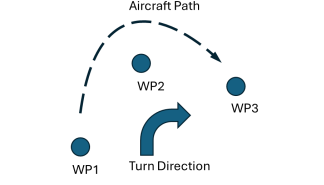
\includegraphics[width=0.65\textwidth]{images/Aircraft path.png}
\caption{The air vehicle shall be capable of automatically navigating around the course defined by
waypoint coordinates, which will be provided by the organisers at the final pre-fly off
webinar.}
\label{fig:navigation}
\end{figure}

\end{itemize}

\section{Aircraft Requirements}
Technical parameters and restrictions affecting aircraft design include:
\begin{itemize}
    \item \textbf{Maximum Take-Off Mass (MTOM):} Must not exceed \textbf{\SI{10.0}{\kilogram}}[T2.2.1]
    \item \textbf{Propulsion:} Electric propulsion only, restricted to standardized \textbf{6s 6000~mAh Li-Po batteries} with XT90 connectors [T2.10, T2.1.1, T2.10]
    \item \textbf{Safety Links:} Two highly visible, externally removable XT90 safety loop links are mandatory (Link 1: isolates avionics, Link 2: isolates propulsion ESCs) [T3.2.1, T3.2.2 , T3.2.3]
    
    \item \textbf{Weather Resilience:} Must operate in winds up to \SI{20}{\knot} (gusts to \SI{25}{\knot}) and light rain [T2.6.1]
    
    \item \textbf{Contrast:} At least 25\% of the surface area must feature highly contrasting colors relative to green, brown, and yellow vegetation [T2.4.5].

    
    \item \textbf{Storage Box:} Complete system (including aircraft and GCS) must fit inside a box $\le$ \SI{1500}{\milli\meter} $\times$ \SI{600}{\milli\meter} $\times$ \SI{600}{\milli\meter} [T6.1.1 , T6.1.2 , T6.1.3]

    \item \textbf{Assembly:} Routine toolless assembly from stowed to flight readiness must occur in $\le$ \textbf{\SI{8}{\minute}}
    [F3.4.2]



\end{itemize}

\section{Comparison With Lycans' Competitions}
The UAS Challenge is compared side-by-side with our previous competitions, AIAA Design/Build/Fly (DBF) and the ICMTC UAV Challenge, in Table~\ref{tab:comparison} and Figure~\ref{fig:mtom_comparison}.

\begin{table}[H]
\centering
\caption{Cross-Competition Parameters and Engineering Constraints}
\label{tab:comparison}
\begin{tabular}{llll}
\toprule
\textbf{Parameter} & \textbf{IMechE UAS Challenge 2026} & \textbf{AIAA Design/Build/Fly (DBF)} \\
\midrule
\textbf{Mission Focus} & Autonomous agricultural spraying & Varying annual cargo missions\\
\textbf{Control Format} & Autonomous flight (Manual override) & Strictly Manual RC Pilot  \\
\textbf{Battery Limit} & Standardized 6s 6000~mAh Li-Po & Variable chemistry/weight caps\\
\textbf{Scoring Strategy} & Linear points + Innovation bias & Multiplicative efficiency formula \\
\textbf{Payload Type} & Liquid water (precise release) & Solid weights / folding structures \\
\textbf{Structural Box} & Box $\le 1500 \times 600 \times 600$\,mm & Wingspan / folding limits  \\
\bottomrule
\end{tabular}
\end{table}

\begin{table}[H]
\centering
\caption{Cross-Competition Parameters and Engineering Constraints}
\label{tab:comparison}
\begin{tabular}{llll}
\toprule
\textbf{Parameter} & \textbf{IMechE UAS Challenge 2026}  & \textbf{ICMTC UAV Challenge} \\
\midrule
\textbf{Mission Focus} & Autonomous agricultural spraying & Target reconnaissance \\
\textbf{Control Format} & Autonomous flight (Manual override)  & Autonomous waypoint flight \\
\textbf{Battery Limit} & Standardized 6s 6000~mAh Li-Po & Typically unconstrained \\
\textbf{Scoring Strategy} & Linear points + Innovation bias  & Mission precision + Reviews \\
\textbf{Payload Type} & Liquid water (precise release) & Gimbal camera payloads \\
\textbf{Structural Box} & Box $\le 1500 \times 600 \times 600$\,mm &  Military-ruggedized standards \\
\bottomrule
\end{tabular}
\end{table}


\begin{thebibliography}{9}
\bibitem{rules_ref}
Institution of Mechanical Engineers (IMechE), \emph{IMechE UAS Challenge 2026 Competition Rules}, Version 4, released September 12, 2025.
\bibitem{news_ref}
UAS Challenge Organising Committee, \emph{UAS Challenge 2026 rules released}, IMechE Aerospace Division, 12 September 2025.
\end{thebibliography}

% ============================================================
% APPENDIX: OTHER COMPETITIONS
% ============================================================
\section*{Appendix: Additional Aerodesign Competitions}
The following regional and international events represent alternate design envelopes and flight validation environments:



\begin{description}[leftmargin=1.5em, labelindent=0em]
    \item[\color{LycansBlue}SAE Aero Design:] Evaluates heavy-lift capabilities, structural safety, and payload optimization. 
    \\ \textbf{Resources:} \href{https://www.saeaerodesign.com/cdsweb/reg/Upcomingcomplist.aspx}{Official Registration} $\cdot$ \href{https://aerouw.org/rule_summary.pdf}{Rulebook Summary}
    
    \item[\color{LycansBlue}TEKNOFEST Inter-High School UAV:] Focuses on design and flight performance tasks optimized for youthful aerospace engineers.
    \\ \textbf{Resources:} \href{https://teknofest.org/en/competitions/inter-high-school-unmanned-aerial-vehicles-competition/}{TEKNOFEST Website} $\cdot$ \href{https://cdn.teknofest.org/media/upload/userFormUpload/2026_\%C4\%B0HA_Yar\%C4\%B1\%C5\%9Fmalar\%C4\%B1_\%C5\%9Eartnamesi_EN_v6_TnAKT.pdf}{Rulebook (EN v6)}
    
    \item[\color{LycansBlue}IMechE UAS Challenge:] Focuses on autonomous flight navigation, payload delivery, and ground assembly.
    \\ \textbf{Resources:} \href{https://www.imeche.org/news/news-article/uas-challenge-2026-rules-released}{Competition News} $\cdot$ \href{https://www.imeche.org/docs/default-source/1-oscar/challenges/uas-challenge/uas-2026/260319-uas-2026-rules-v4.pdf?sfvrsn=2}{2026 Rule Book}
    
    \item[\color{LycansBlue}IARC (International Aerial Robotics Competition):] Tackles state-of-the-art robotic behaviors that are currently impossible for commercial or military systems.
    \\ \textbf{Resources:} \href{http://www.aerialroboticscompetition.org/}{IARC Website} $\cdot$ \href{http://www.aerialroboticscompetition.org/assets/downloads/mission10rules_3.1.2.pdf}{Mission 10 Rules}
    
    \item[\color{LycansBlue}C-UASC (California UAS Competition):] Regional challenge targeting search-and-rescue (SAR) capabilities and waypoint tracking under rigorous geographic constraints.
    \\ \textbf{Resources:} \href{https://www.calstatela.edu/ecst/c-uasc}{C-UASC Website} $\cdot$ \href{https://www.calstatela.edu/sites/default/files/C-UASC\%202026\%20Competition\%20Rules\%20rev\%203\%202026-02-23_accessible.pdf}{2026 Rulebook}
    
    \item[\color{LycansBlue}FAI Aeromodelling Commission (CIAM):] The global governing body setting international aeromodelling standards and championship rules.
    \\ \textbf{Resources:} \href{https://www.fai.org/commission/ciam}{CIAM Home Page}
    
    \item[\color{LycansBlue}SUAS (Student Unmanned Aerial Systems):] Challenges teams to build a system capable of autonomous navigation, object detection, and obstacle avoidance.
    \\ \textbf{Resources:} \href{https://robonation.gitbook.io/suas-resources}{SUAS Resource GitBook}
    
\end{description}

\end{document}